\chapter{Neural Network Noise Suppression}\label{NeuralNetworkNoiseSuppression}
In this section the Machine learning approach will be explained.
This method will be used to suppress the noise from the signal, keeping the speech as clean as possible.

\section{Artificial Neural Network Theory}

An Artificial Neural Network is a a machine learning technique or computing system that slightly resembles a brain and its neuronal connections. Being programmed without specific rules, an ANN system has one or more layers of artificial neurons with specific weights associated to each one of them. By giving the system multiple input sequences, it will \"train\" itself by adjusting the weights to have an output prediction that will resemble the wanted output as much as possible.

\subsection{Artificial  Neurons}

An artificial neuron is an elementary unit in an artificial neural network. As being inspired by biological neurons, their purpose is to simulate the different function that they have:
\begin{itemize}
\item Gathering all the inputs
\item Multiplying with their each individual weight
\item Adding all the weighted inputs
\item The sum will be passed to the activation function
\item Outputting the result
\end{itemize}

\begin{figure}[htp]
	\centering
	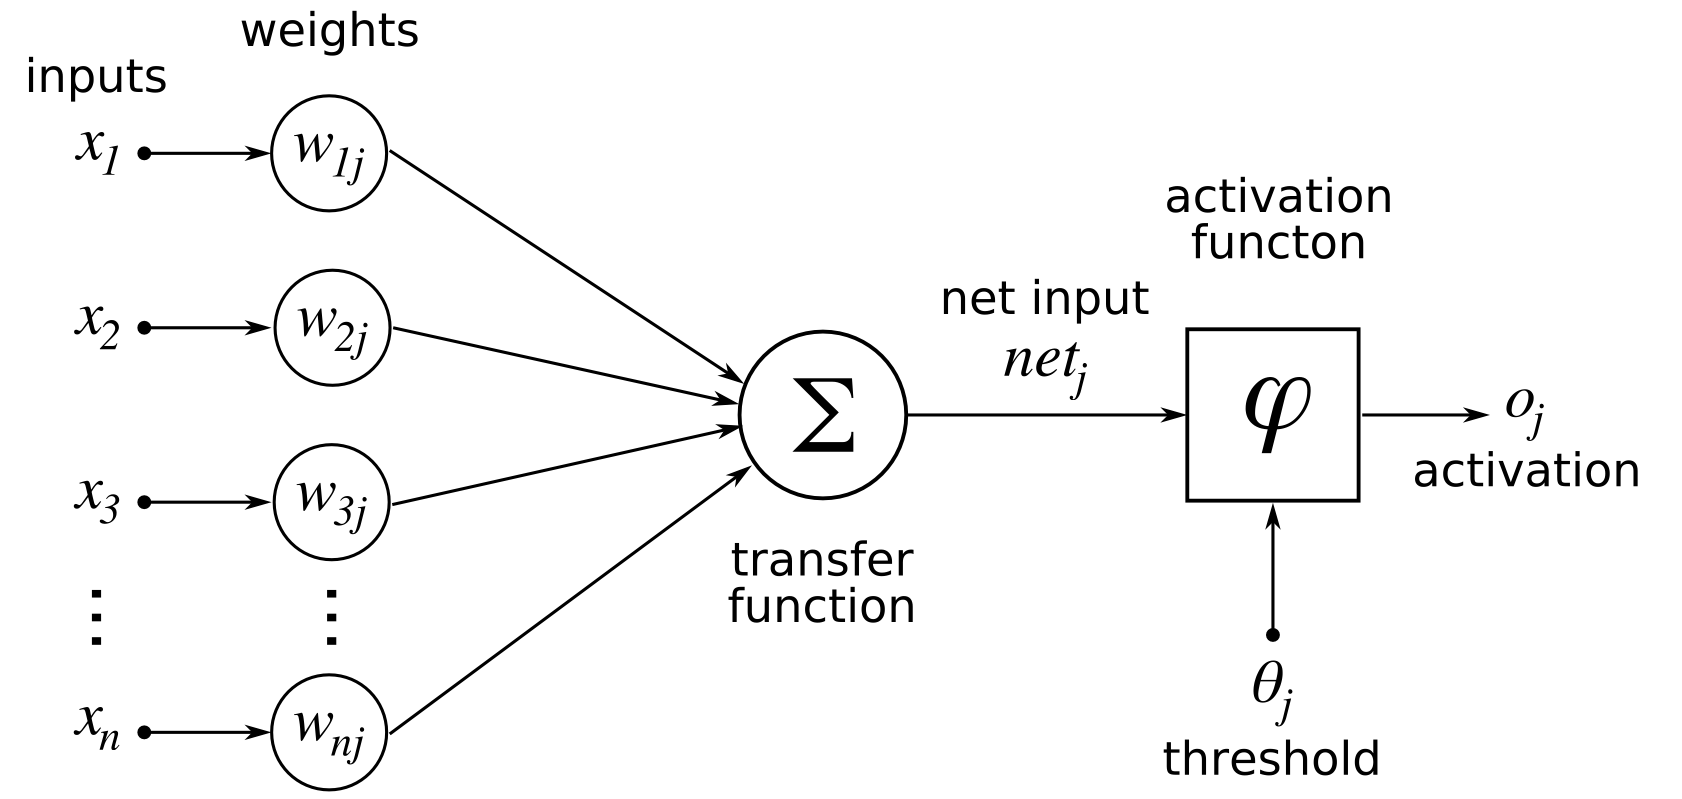
\includegraphics[width=1\textwidth]{Illustrations/artificialneuron.png}
	\caption{Example of an Artificial Neuron}
	\label{fig:ArtificialNeuron}
\end{figure}

In figure \todo{add nr of figure}, representing an artificial neuron, all those functions can be seen. The neurons will be received, multiplied by a vector of weights, added together and sent to the activation function which will then give the output of the artificial neuron.

\subsection{Activation Functions}

As stated in the last section, each neuron will have an activation function. Being biological inspired, it usually represents the rate of action potential in the cell, depending on the range and the case, this can be from 0 to 1 or from -1 to 1. In the range of 0 to 1, which resemble the biological neuron more, this can be seen as the neuron firing or not.

Two of the most used activation function are:
The sigmoid Function:

\begin{itemize}
\item The sigmoid Logistic Function: Which maps the input from 0 to 1.This can be really useful where neurons have to predict the probability as the output.
\begin{equation}
 \sigma(z) = \frac{1}{1+e^{-z}}
\end{equation}

\item Hyperbolic tangent function: Which maps the input from -1 to 1. This can be used when the classification between two classes is needed.
\begin{equation}
 \phi(z) = tanh(z)= \frac{2}{1+e^{-2x}}-1
\end{equation}

\end{itemize}

\begin{figure}[htp]
	\centering
	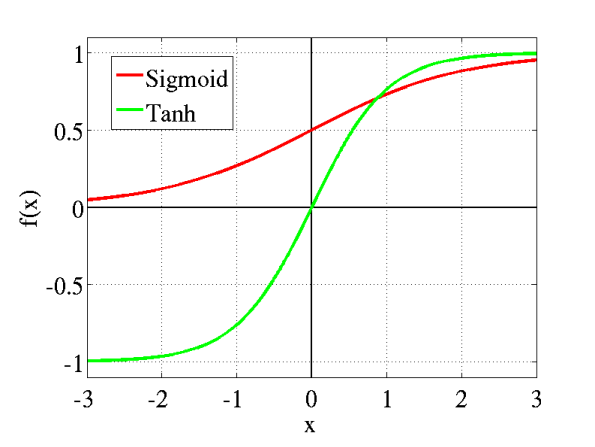
\includegraphics[width=0.5\textwidth]{Illustrations/sigmoidandtangent.jpeg}
	\caption{Both sigmoid and tangent functions exemplified}
	\label{fig:SigmoidAndTangent}
\end{figure}

\subsection{Types of Artificial Neural Networks}

\subsubsection{Feed-Forward Networks}

The feed-forward neural network is one the first methods invented and one of the simplest. As the name suggests, the information moves only forward from the input, through the hidden layers is it has any, to the output. All neurons are directly connected to the neurons from the next layer, they have no cycles or loops like other other neural networks that are going to be presented.

Different types exists, as single layer perceptron, which have the inputs being fed directly in the output layer using a series of weights. Multi-layer perceptron is another one, which,compared with the single layer perceptron, has one or more hidden layers of neurons.
In most cases a sigmoid activation function is going to be used for those types of neurons as they are usually used for classification purposes.In other types like Convolution neural networks,which are composed of one or more convolutional layers, have fully connected layers, meaning that all the lengths of the output vector will be equal with the input one.

\subsubsection{Recurrent Neural Networks}

Recurrent Neural Networks are is an artificial neural network model which uses sequential information. In other models, like feed-forward networks, all the input and outputs are independent of each other, meaning that one series of inputs cannot affect the result of others.
This can be really useful in some cases like translation, speech recognition, sound optimization, text prediction, where giving an output based on past iterations can be more precise and easier or even completely necessary in some cases.

\newpage
\subsubsection{Gated Recurrent Unit Networks} 

Gated Recurrent Unit Networks are a type of recurrent neural networks firstly introduced by Kyunghyun Cho et al in 2014.\todo{add references all over the place} similar to LSTM networks but with fewer parameters, it has shown better results then LSTM in some cases. Usually used and with a good performance on speech signal modulation, music modelling and noise suppression, GRU networks will be one of the main network types that will be used in the building of our neural network.

\begin{figure}[htp]
	\centering
	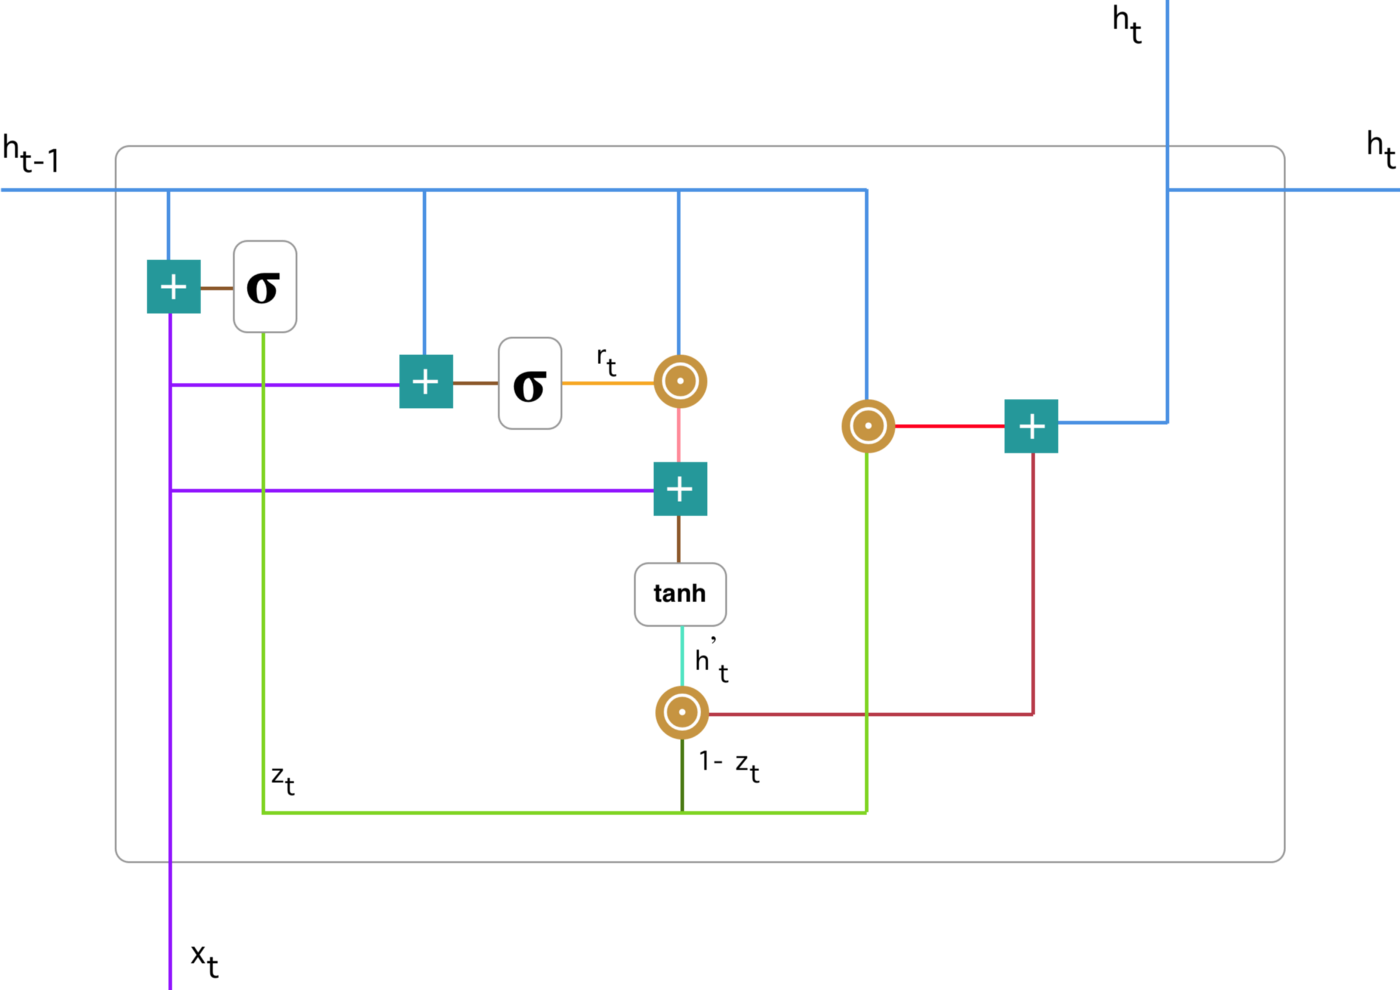
\includegraphics[width=0.7\textwidth]{Illustrations/GRU.png}
	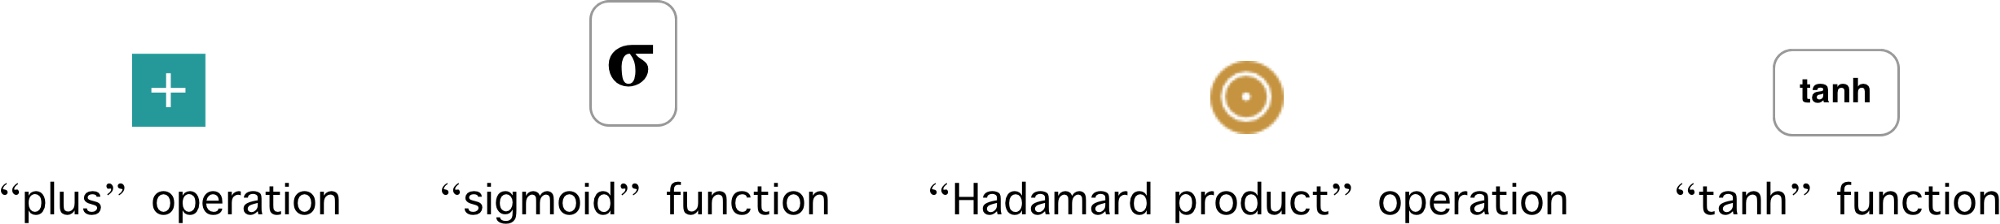
\includegraphics[width=0.7\textwidth]{Illustrations/GRUsymbols.png}
	\caption{Example of a single Gated Recurrent Unit}
	\label{fig:GRU}
\end{figure}


GRU, compared with RNN has an update gate and a reset gate, which solves one problem that RRN had: the vanishing gradient problem. This is a problem that mostly happends with very deep neural networks, in which because of the way the gradient-based learning method works, the gradient can became really small or even disappear which will make the training very slow or even incapacitate the neural network and basically stop the training process not letting any weights being updated.


\begin{figure}[htp]
	\centering
	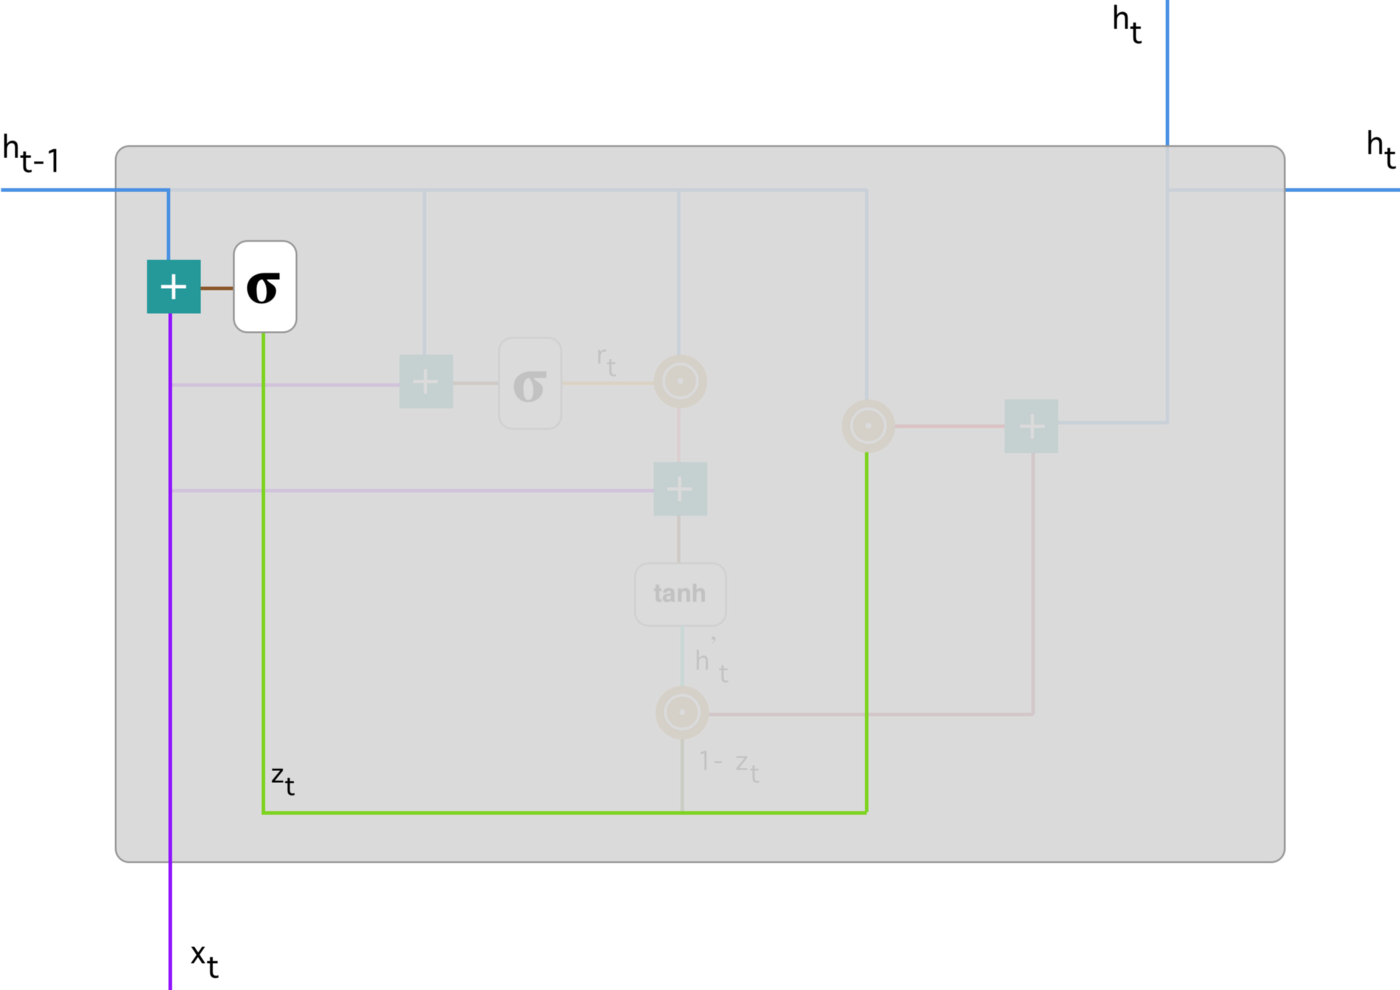
\includegraphics[width=0.7\textwidth]{Illustrations/GRUupdategate.png}
	\caption{The update gate exemplified in the unit}
	\label{fig:GRUupdategate}
\end{figure}


\subsubsection{The Update Gate}

First operation made in the unit will be the calculation of the Update gate.
\begin{equation}
  z_t =\sigma(W^{(z)}x_t + U^{(z)}h_{(t-1)})
\end{equation}

As exemplified in figure \todo{add figure nr} both $x_t$ and $h_{t-1}$,which hold information from the last $t-1$ unit, will be multiplied by respective weights, $W^{(z)}$ and $U^{(z)}$ respectively. The results will be summed together and a sigmoid activation function is going to limit their range between 0 and 1.

This is a really important part of the unit as it will determine how much of the past values will be taken in consideration and passed for future calculations. By doing this, the unit can remember a lot of steps in the past and eliminate the vanishing gradient problem had before in RNN networks.

\begin{figure}[htp]
	\centering
	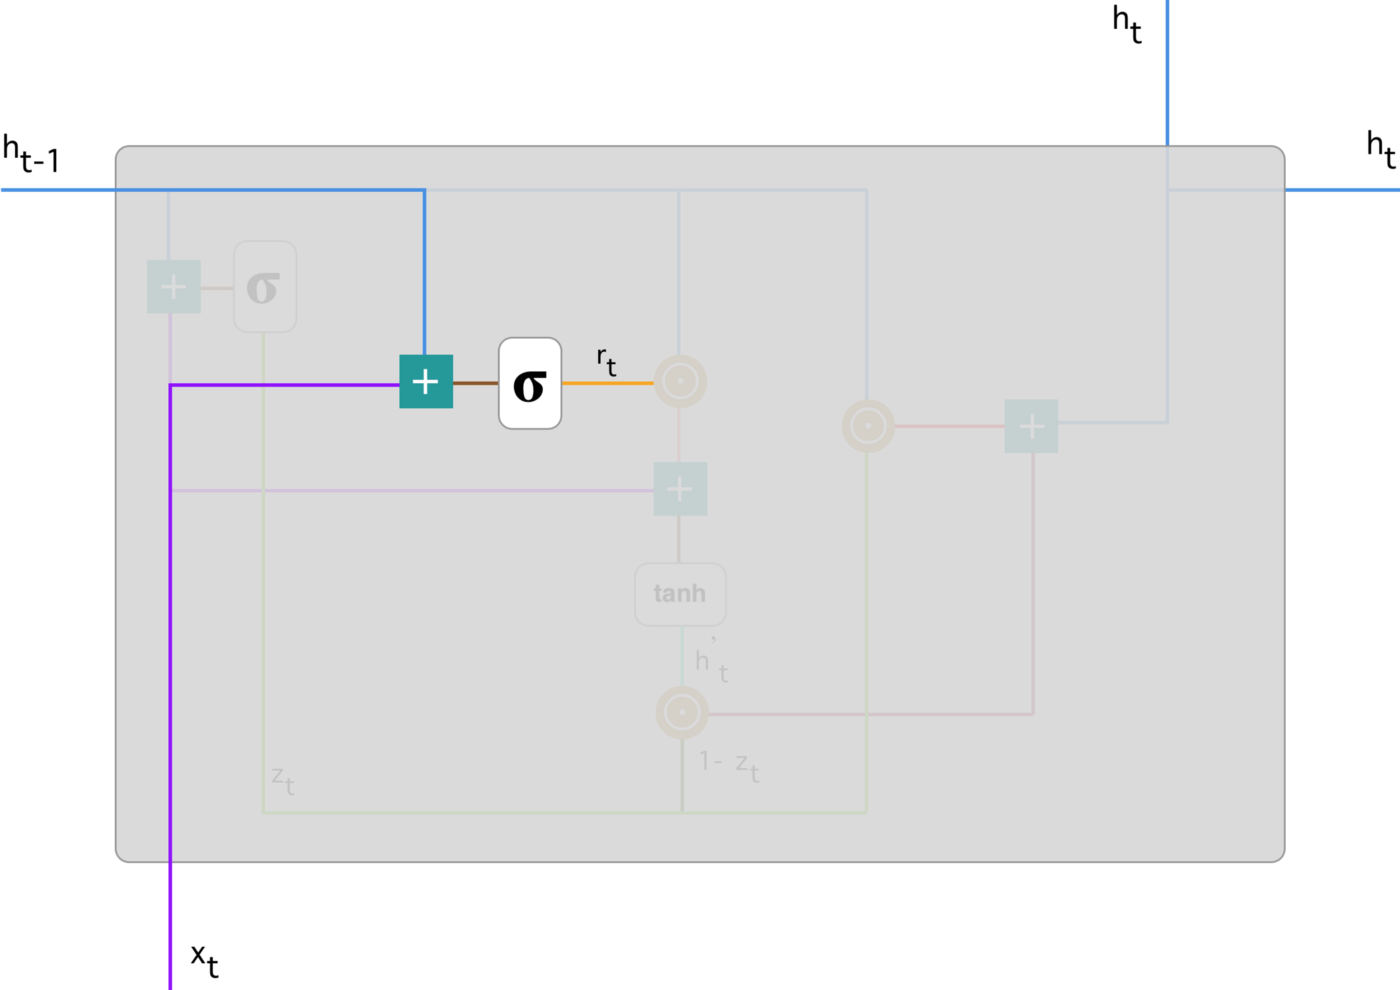
\includegraphics[width=0.7\textwidth]{Illustrations/GRUresetgate.png}
	\caption{The Reset Gate exemplified in the unit}
	\label{fig:GRUresetgate}
\end{figure}

\subsubsection{The Reset Gate}
The reset gate, compared with the update gate, will calculate how much of the past data to let go.
\begin{equation}
r_t=\sigma(W^{(r)}x_t+U^{(r)}h_{t-1})
\end{equation}
The formula is quite similar to the one from the update gate, the difference being in the weights used and the usage of the results in figure\todo{add nr of figure} we can see the same lines being used as in the update gate to gather data, multypling them with the weights, adding the results together and passing them to a sigmoid activation function.

\subsubsection{Present memory}

\begin{figure}[htp]
	\centering
	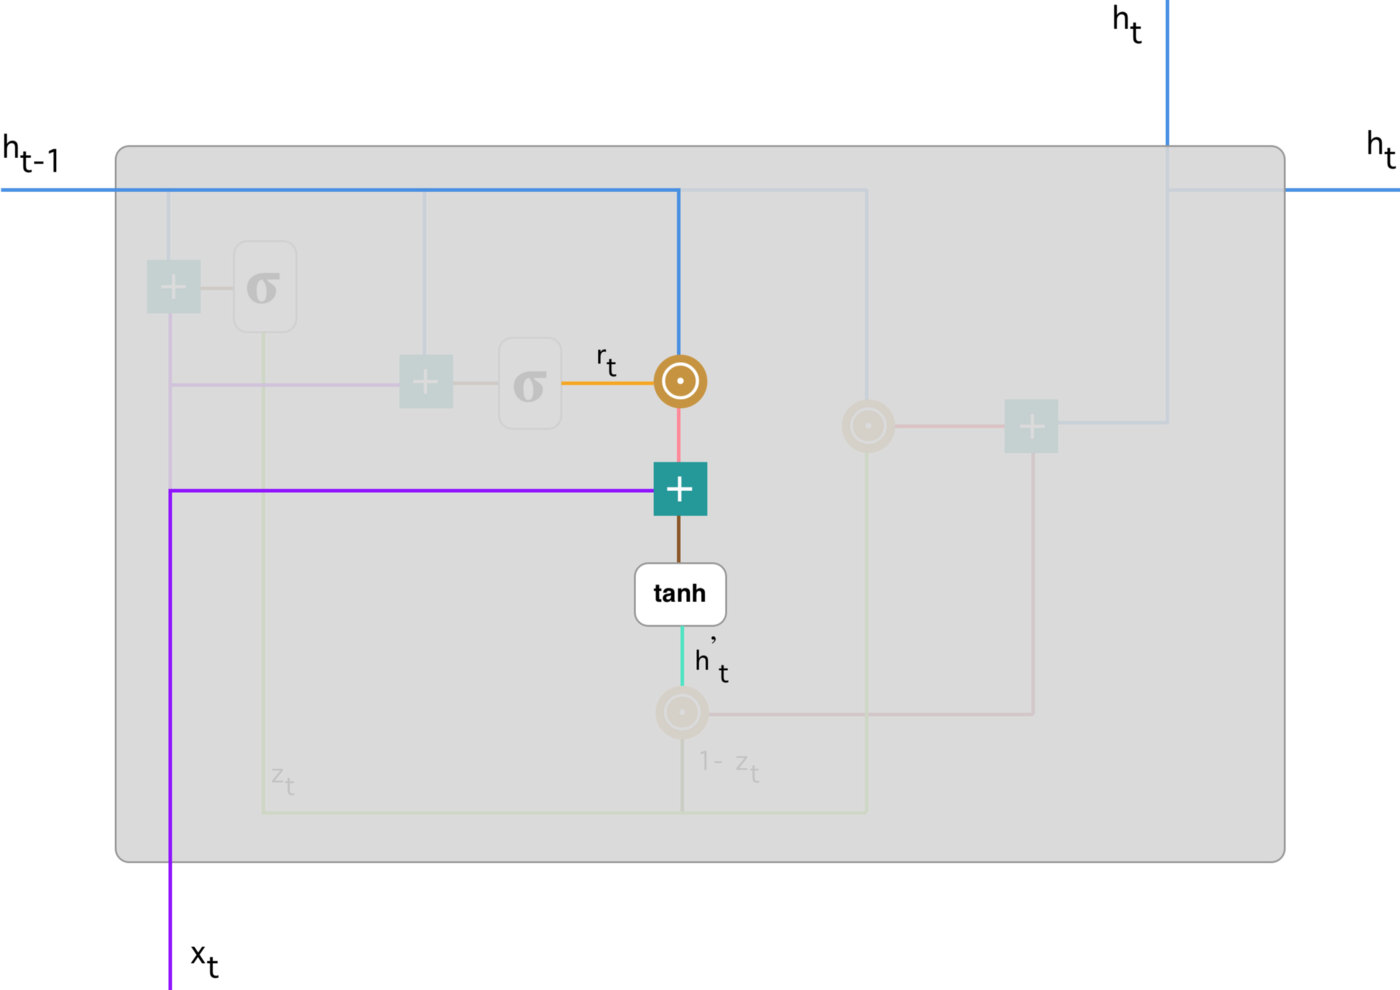
\includegraphics[width=0.7\textwidth]{Illustrations/GRUpresentmemory.png}
	\caption{Present memory calculation step in the unit}
	\label{fig:GRUpresentmemory}
\end{figure}

After calculating the gates, in the next two steps the final result will be calculated.
Firstly the reset gate will be used to store usable information from the past in the present memory content.
\begin{equation}
h'_t=tanh(Wx_t+r_t \circ Uh_{t-1})
\end{equation}

Firstly the input $x_t$ and $h_{t-1}$ will be multiplied with their weights: $W$ and $U$ respectively. The element wise or Hadamard product will be taken between the reset gate $r_t$ and $Uh_{(t-1)}$.This will basically determine how much to remove from the past time steps. After that the results will be added together and passed to a tanh activation function.

\subsubsection{Final memory at present time}

\begin{figure}[htp]
	\centering
	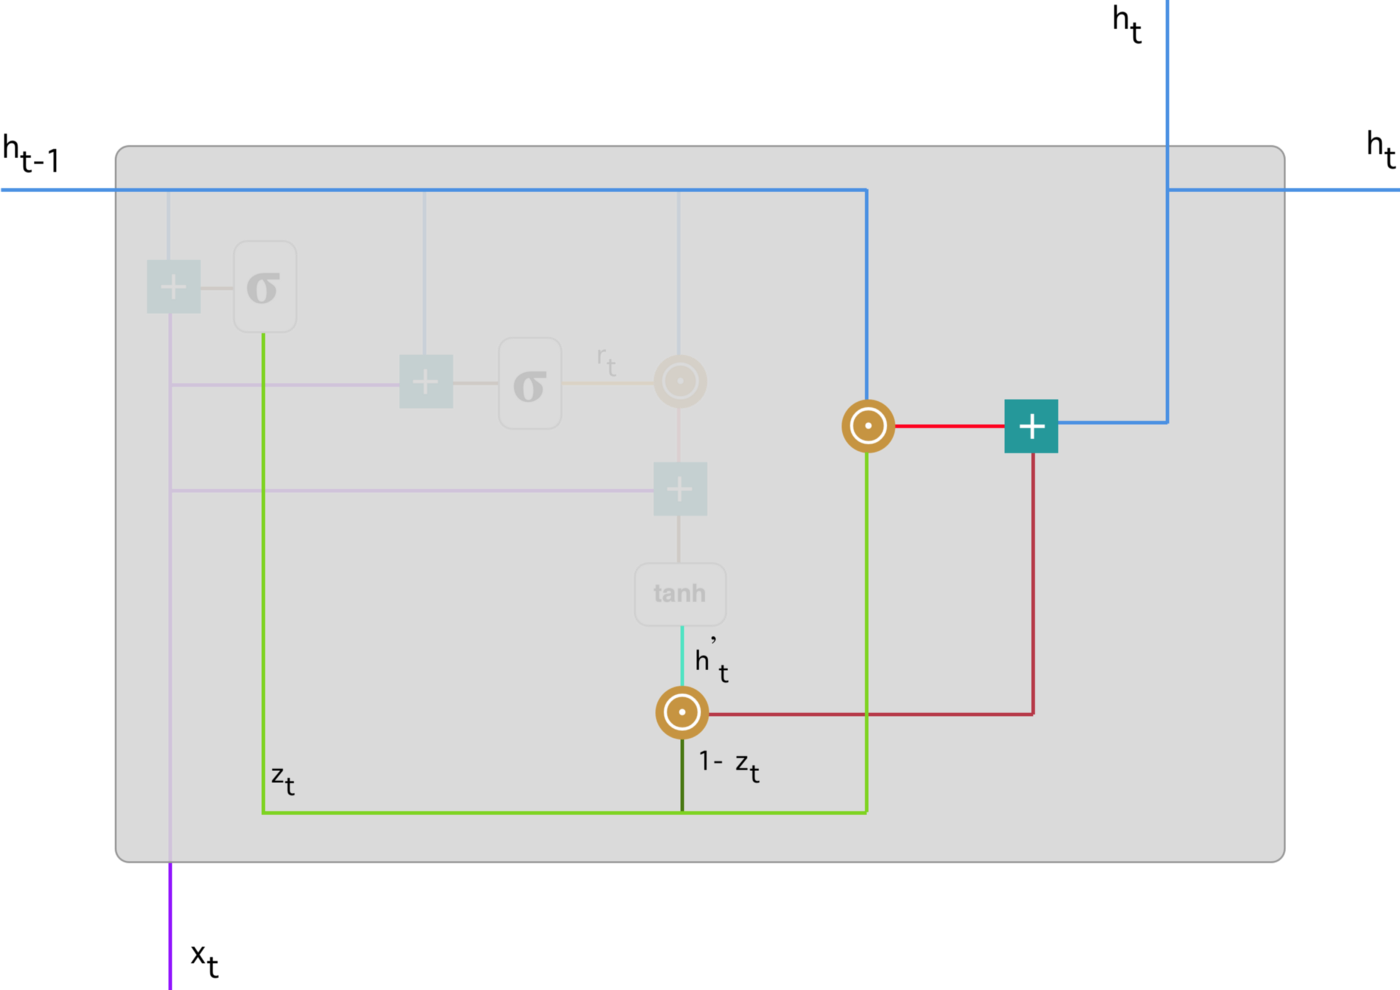
\includegraphics[width=0.7\textwidth]{Illustrations/GRUlaststep.png}
	\caption{Final memory at present time calculation in the unit}
	\label{fig:GRUlaststep}
\end{figure}

In the last part of the gated recurrent unit, the new $h_t$ has to be calculated, which will hold the information for the current unit and pass it to the rest of the network.
Now the update gate will be used to determine what to use from $h'_t$ current step and from the previous step $h_{(t-1)}$.

\begin{equation}
h_t=z_t \circ h_{t-1}+(1-z_t) \circ h'_t
\end{equation}

Firstly the gate $z_t$ and $h'_t$ will be multiplied element-wise, then $(1-z_t)$ and $h'_t$ will be multiplied element-wise also. The sum of those results will be the end result $h_t$. 

Finally the end result, and the whole gated recurrent unit unfolded will look as in figure \todo{add figure nr}

\begin{figure}[htp]
	\centering
	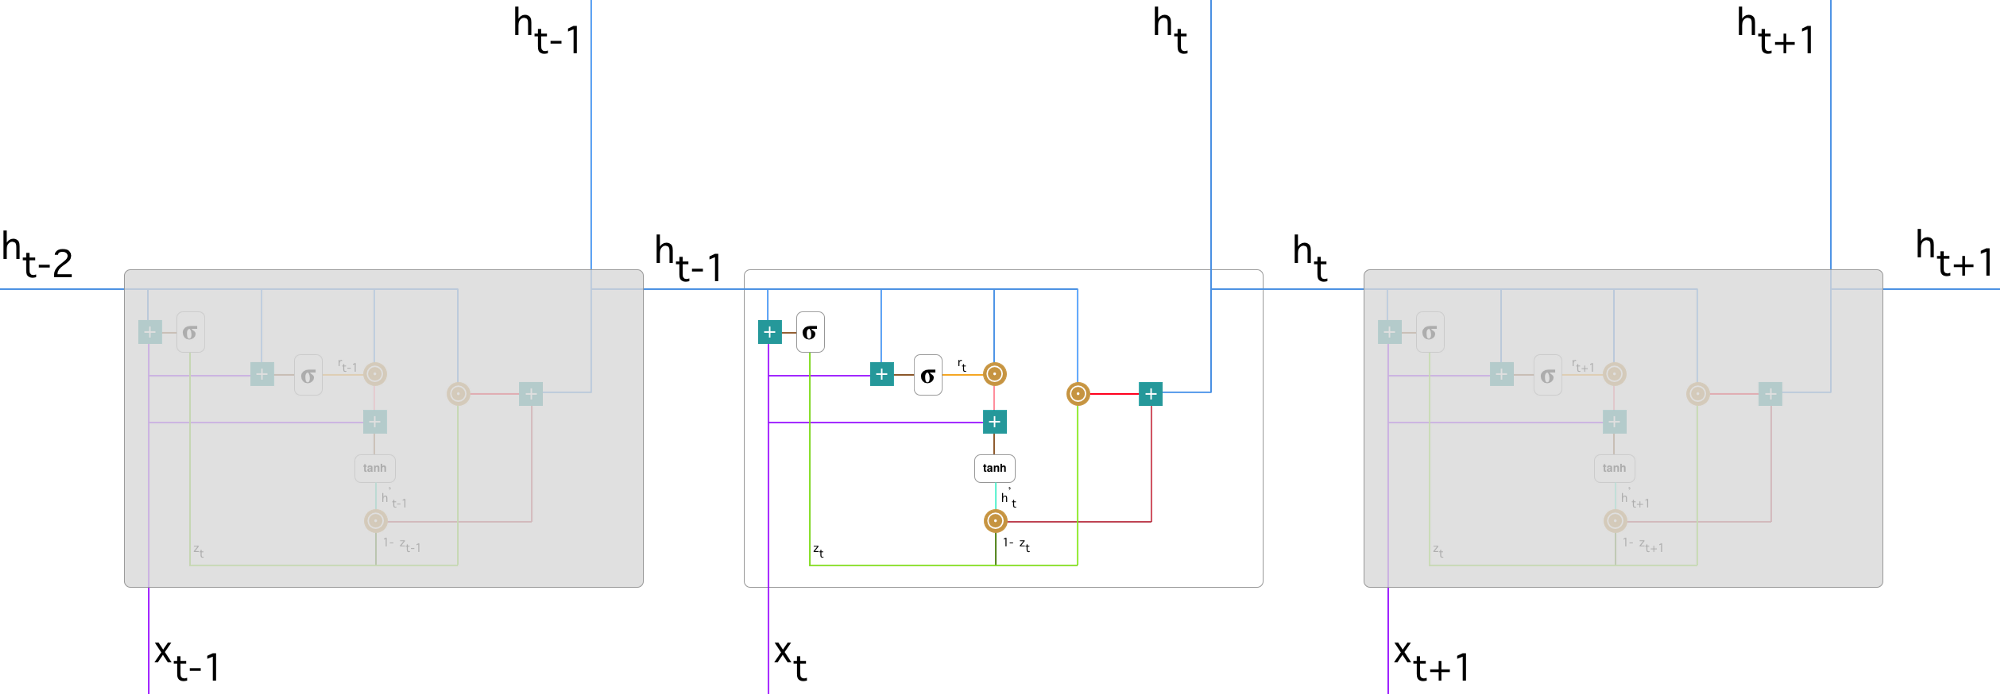
\includegraphics[width=0.7\textwidth]{Illustrations/GRUunfolded.png}
	\caption{The GRU unfolded with the past,present and future units}
	\label{fig:GRUunfolded}
\end{figure}

\subsubsection{Bidirectional Recurrent Neural Networks} 
As mentioned, Recurrent neural networks are capable of are able to recall features from past states of the network but with a Bidirectional recurrent neural network the layer will be able to calculate the next state using both past and future states information. This is done by having two hidden recurrent neural network layers that with opposite directions connected together and to the same output. 

\begin{figure}[htp]
	\centering
	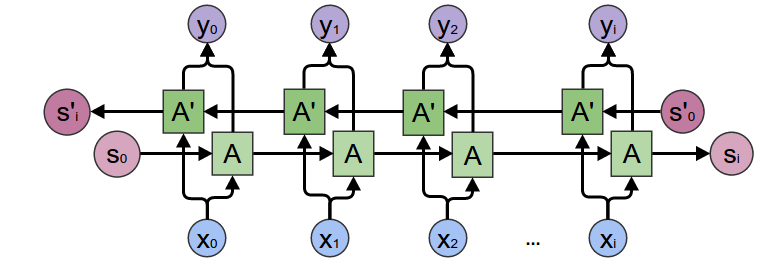
\includegraphics[width=0.7\textwidth]{Illustrations/BRNN.png}
	\caption{A bidirectional recurrent neural network layer exemplifying the directional neurons}
	\label{fig:BRNN}
\end{figure}

As seen in figure \todo{add figure nr.} the two layers get the same input and send the same output but the directions of the neurons are opposite.

This can be helpful in a multitude of cases as translation, handwriting recognition or, specific to our case, speech recognition and noise elimination, as in all of those cases, information about both the future and past can be helpful to calculate the present state 
\section{Model Development}

After The sample is filtered with the directional filter, noise from the specified direction will still remain. For that reason the goal of the project was to develop a neural network algorithm that will practically act as an adaptive filter to suppress the remaining noise. The neural network consists mostly of Recurrent neural network layers with Gated Recurrent units as they have been proven to be very effective for this specific case of eliminating noise. Further in the project, variations of the neural network with different layer configurations will be examined to see how they would act on this specific case, and different training methods too to see which will be the most efficient.

\subsubsection{Regularization Methods}
A big problem that can happen while training is over-fitting. By training on a set of data too much, or having a small dataset will result in an over-fitted neural network that will give really good results on data from the dataset, but when tests with new data are made, the prediction of the neural network will be far from the wanted result.


For that reason regularization methods can be used to ensure that the data will not be over-fitted. Those will be some layers in the neural network that will only be active during the training.
One technique used in the project is the Dropout regularization method. This is one of the most effective methods, firtly introduced by Srivastava et al in 2014 \todo{add reference}. This works by giving each neuron a probability to be set to zero, in this way random neurons will be ignored or "dropped out". This works really well as no neuron will over specialize for only one feature, as if that happends, and that specific neuron is dropped out, other neuron will have to make predictions even without that neuron. This, in the end, will result in multiple independent internal representations being learned by the network. Otherwise, the neuron will rely too much on some of the features represented by other neurons and will result in complex co-adaptations.


\begin{figure}[htp]
	\centering
	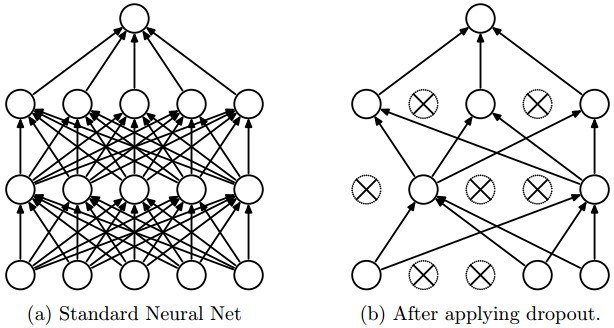
\includegraphics[width=0.7\textwidth]{Illustrations/dropout.jpeg}
	\caption{A representation of the dropout function during training}
	\label{fig:dropout}
\end{figure}

This function can be better seen in figure \todo{add nr of figure}, as after applying dropout only some connections will be kept instead of all of them.
\newpage
\subsection{Data Preprocessing}

For training and evaluating the Neural Network data was needed to create the dataset. As the objective of the neural network is to filter out noise from a noisy speech sample, samples of clean speech and noise were needed. The speech samples were taken from LibriSpeech \todo{add reference http://www.openslr.org/12/}. From there 100 hours of audio books with clean speech were taken.
For the noise, approximately 16 GB of noise were collected in a freely available pack from \todo{add reference https://people.xiph.org/~jm/demo/rnnoise/}.

all this data had to be processed as they come in different formats.
To create a dataset big enough, and to avoid overfitting this process was automated and randomized. Firstly, a random sample of clean speech is taken, which is between 2 and 20 seconds. As most of the noise samples are around 1 minute, a random sample will be chosen, and from that sample a random section of the same length as the speech sample will be taken.

By combining both of the samples the noisy sample that can be used is finished.
The MFCC of both the noisy sample and the clean speech will be calculated as those will serve as the training data and target data respectively.

\begin{lstlisting}[language=Python, caption=Noise sample gathering class]
class noise:
    def __init__(self,size):
        self.size = size
    
    def choose_random(self):
        path = r"C:\Users\Darius\Desktop\sound samples\training data for RNN\rnnoise_contributions"
        files = os.listdir(path)
        index = random.randrange(0, len(files))
        if  files[index].endswith('.txt'):
            index = index -1
        file_path = os.path.join(path, files[index])
        self.sample, fs = sf.read(file_path, channels=2, samplerate=24100,format='RAW', subtype='PCM_16')
        i=0
        while i!=1:
            random_sequence = random.randrange(0,len(self.sample))
            if random_sequence + self.size < len(self.sample):
                i=1
        self.sample = self.sample[random_sequence:]
        self.sample = self.sample[:self.size ,:1]
        self.nfcc   = python_speech_features.mfcc(self.sample,18000,0.025,0.01,24)
        
    def show_sample():
        print(file_path)
        plt.plot(self.sample)
    def listen_sample(self):
        sd.play(self.sample) 

\end{lstlisting}

Here, the class noise will do the whole process described and will be further used in the code to retrieve any parameters for the noise sample.

\subsection{Training methods}
By gathering all the data described, a dataset could have been built, but to combine all the clean speech and noisy data and target dataset too would take a large amount of time, memory and processing power that were not available to us at the time. As even  a dataset of only 1000 samples already used more than 1.5 GB.

Another option then building a large dataset was to use a generator and keras fit.generator() function to train the neural network instead. By doing that, a generator was able to be built that generates data for input and output of the neural network one batch at at time. This would not work in the tradition way as the neural network wouldn't be able to train more than one epoch, but the size of the dataset can be resized indefinitely.

Multiple tests were made to research the reliability of both of those methods.

\todo{add picture of both test}

But as seen in\todo{add nr of figure that need to be added} the test results were inconclusive so we decided to do the further tests with a more traditional approach of using a constructed dataset.


The dataset used contains 1000 samples for training and 400 samples for validation (roughly 30\%).All the samples consists of varying noise,speech samples and length to not overfit the neural network on specific parameters.
Table \ref{tab:firsttable} represents the batch size, dropout, learning rate, epochs and samples used for each model.
All the models from the table are further discussed in the next section.

\begin{table}[htp]
\centering
\begin{tabular}{|c|c|c|c|}
\hline
Parameters         & Model 1 & Model 2 & Model 3 \\ \hline
Batch Size         & 20      & 20      & 20      \\ \hline
Dropout            & 0.15    & 0.15    & 0.15    \\ \hline
Learning Rate      & 0.001   & 0.001   & 0.001   \\ \hline
Training Samples   & 1000    & 1000    & 1000    \\ \hline
Validation Samples & 400     & 400     & 400     \\ \hline
Epochs             & 30      & 30      & 30      \\ \hline
\end{tabular}
\caption{Same Parameters Used On All Models}
\label{tab:firsttable}
\end{table}
Another note that could be made is that instead of using a classical stochastic gradient descent, as the optimization algorithm, adam(Adaptive moment estimation) was used which have some good benefits of being quite low on memory usage, is computationally efficient and and is appropriate for non-stationary objectives.
\subsection{Comparison Between Different Models}

In order to have a more optimized model, three neural network models were created and compared to assess their efficiency for our particular case. The training parameters are the same as discussed  in the last section in order to have a proper comparison between them.


The first model consists of two GRU layers and a fully connected layer as seen in Figure \ref{fig:firstModel}.
\begin{figure}[htp]
	\centering
	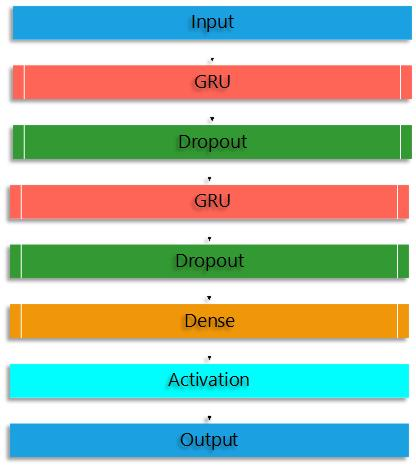
\includegraphics[width=0.5\textwidth]{Illustrations/Model1.jpg}
	\caption{First Model}
	\label{fig:firstModel}
\end{figure}

In the second model the two GRU layers were replaced by a Bidirectional GRU layer followed again by a fully connected layer as seen in Figure \ref{fig:secondModel}.
\begin{figure}[htp]
	\centering
	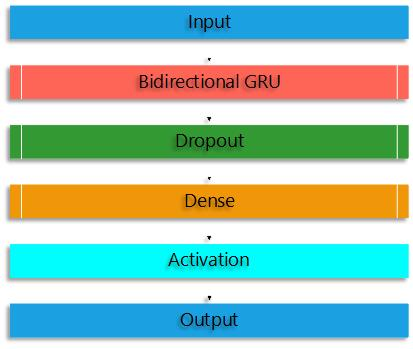
\includegraphics[width=0.5\textwidth]{Illustrations/Model2.jpg}
	\caption{Second Model}
	\label{fig:secondModel}
\end{figure}

For the third model we decided to make a deeper model by adding another fully connected layer before the bidirectional GRU layer as seen the in the figure \todo{add figure nr}. Compared to model one and two , in model three a dropout function was added on the fully connected layers as well.
\begin{figure}[htp]
	\centering
	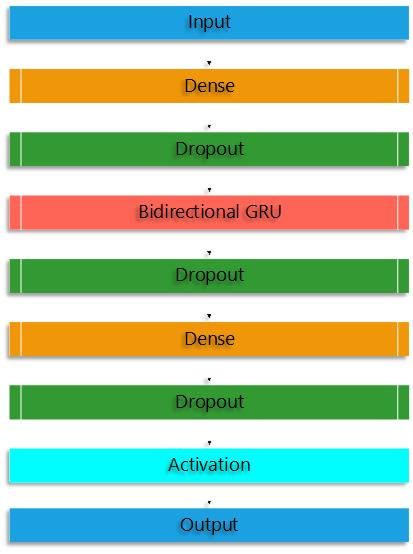
\includegraphics[width=0.5\textwidth]{Illustrations/Model3.jpg}
	\caption{Third Model}
	\label{fig:thirdModel}
\end{figure}





\subsection{Restults for NN}




